\documentclass{exam}
\usepackage{tikz}
\usetikzlibrary{decorations.pathmorphing}

\pagestyle{headandfoot}
\firstpageheader{Name:\underline{\hspace{100pt}}}{}{Date:\underline{\hspace{100pt}}}
\runningheader{}{\textbf{The Aetherius Olympiad in Mathematics}}{}
\firstpagefooter{}{\thepage}{}
\runningfooter{}{\thepage}{}

\begin{document}

\begin{center}
    \LARGE{\textbf{The Aetherius Olympiad in Mathematics}}

    \vspace{8pt}

    \large{2024-09}
\end{center}

\section*{Instructions}

\begin{itemize}
    \item You must immediately fill out your name as well as the current date on the top of the page.
    \item You will be given 30 minutes to complete 3 questions. No extra time is allowed, and one must stop writing as soon as the time is up.
          % \item You will have to show adequate work to prove that your answer was the result of thoughts but not guesses or anything else.
          % \item You must explicitly indicate what your final answer is (\textit{e.g.} circling, boxing, etc).
    \item One would be awarded marks based on not only the right answer, but also on the attempt, logic, and thought. A mere correct answer may not necessarily earn full marks.
    \item Scratch paper would be provided upon request. One may not use their own scratch paper.
    \item You may begin as soon as the timer starts.
\end{itemize}

\section*{Questions}

\begin{questions}
    \question[5]{There are two villages on one side of the river. One person from village A wants to go fishing at the river front, then go to village B to visit his friend. The direct distance from village A to the river is $250m$ and from village B to the river is $360m$. What is the minimum distance that person has to travel? Let the horizontal distance between A to B be $500m$.

        \begin{center}
            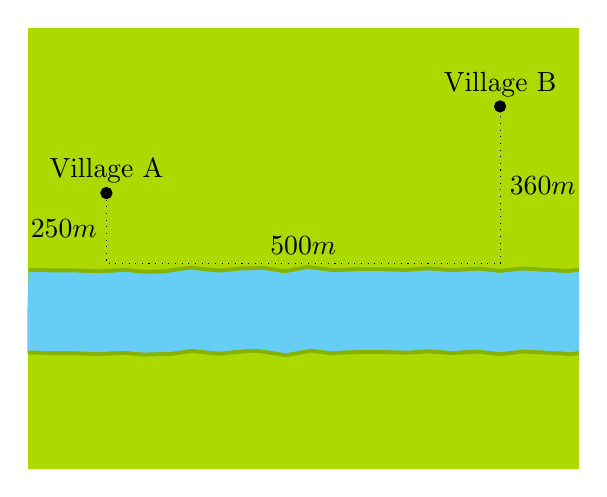
\begin{tikzpicture}
                \coordinate (LB) at (-1,-1);
                \coordinate (LT) at (-1,4.6);
                \coordinate (RB) at (6,-1);
                \coordinate (RT) at (6,4.6);
                \coordinate (Village A) at (0,2.5);
                \coordinate (Village B) at (5,3.6);

                \clip(LB)rectangle(RT);
                \fill[lime!70!olive] (LB)rectangle(RT); % background
                \pgfmathsetseed{14159}
                \draw[decorate, decoration={random steps, segment length=3mm, amplitude=1pt}, lime!70!black, line width=.5mm, double=cyan!60!white, double distance=1cm] (-1,1) -- (9,1); % river
                \draw[black, dotted] (Village A)--node[left]{$250m$}(0,1.6)--node[above]{$500m$}(5,1.6)--node[right]{$360m$}(Village B);
                \filldraw[black] (Village A) circle (2pt) node[anchor=south]{Village A};
                \filldraw[black] (Village B) circle (2pt) node[anchor=south]{Village B};
            \end{tikzpicture}
        \end{center}
    }
\end{questions}

\end{document}